\chapter{Metodología}
\label{chap:metodologia}

En este capítulo se expone de manera concisa la estructura y los principios que han regido el desarrollo de la metodología empleada en este trabajo. Se describe un flujo de trabajo totalmente automatizado —o \emph{pipeline}— que abarca desde la generación de combinaciones de compilación hasta la obtención de métricas y la producción de informes y gráficas. Gracias a su diseño modular, este proceso permite evaluar sistemáticamente cómo distintos compiladores, niveles de optimización y \emph{flags} de seguridad afectan al rendimiento, al tamaño del binario y al grado de fortificación de las funciones. Finalmente, se detallan los programas sobre los que se ha aplicado el análisis y los criterios adoptados para la representación visual de los resultados, con el objetivo de facilitar la interpretación y comparar de forma clara las diferentes combinaciones.


\section{Descripción general del proceso}

Para llevar a cabo el análisis, se ha desarrollado un \emph{pipeline}
automatizado que permite compilar, ejecutar y evaluar de forma
sistemática un conjunto de programas fuente, utilizando distintos
compiladores y combinaciones de \emph{flags} de seguridad y
optimización.

El flujo del proceso se divide en tres etapas principales:

\begin{description}
    \item[\textbf{Entrada:}] 
    Se parte de programas escritos en C++ y Rust. Para cada uno, se
    generan múltiples configuraciones mediante la combinación de
    diferentes opciones de seguridad y niveles de optimización. Estas
    combinaciones se aplican por separado en tres compiladores:
    \emph{GCC}, \emph{Clang} y \emph{Rustc}.

    \item[\textbf{Proceso:}]
    Cada configuración se compila y ejecuta múltiples veces para obtener
    métricas estables. Durante las ejecuciones, se recogen automáticamente 
    datos sobre el tiempo de ejecución, el uso de memoria, el tamaño final 
    del archivo ejecutable (o binario) y el porcentaje de funciones fortificadas detectadas.

    Los datos se almacenan inicialmente en ficheros de texto y
    JSON como salida bruta. A partir de estos ficheros, se
    genera un informe estructurado en formato PDF para cada
    compilador, que organiza los resultados de forma clara para su lectura
    directa.

    Posteriormente, se ejecutan scripts que transforman esa información en
    un conjunto de gráficas automáticas, también en formato PDF,
    que permiten ver las comparaciones de forma más efectiva.

    \item[\textbf{Salida:}]
    La salida final del \emph{pipeline} incluye informes de texto y 
    JSON: con los datos sin procesar, informes PDF que presentan 
    los resultados estructurados y explicados para cada compilador, y gráficas
    PDF que muestran comparaciones entre compiladores, 
    \emph{flags} de seguridad y niveles de optimización, permitiendo
    detectar patrones y diferencias de forma intuitiva.
    
\end{description}


La Figura \ref{fig:flujo_pipeline} muestra el flujo del pipeline creado. Este diseño modular y automatizado garantiza que los resultados puedan
obtenerse fácilmente si se añaden nuevos programas o configuraciones, y
permite centrarse en el análisis y la interpretación de resultados.

\begin{figure}[htbp]
  \centering
  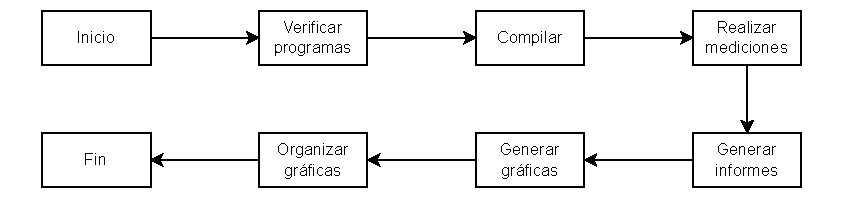
\includegraphics[width=\textwidth]{Pipeline_pro.pdf}
  \caption{Flujo de la pipeline}
  \label{fig:flujo_pipeline}
\end{figure}

\section{Programas utilizados}

Los programas seleccionados están diseñados para revelar de
forma clara el impacto de las medidas de seguridad y de las
optimizaciones aplicadas. Incluyen operaciones básicas sobre memoria,
uso de funciones estándar susceptibles de fortificación, y estructuras
de control simples. Esta elección permite centrarse en los efectos que
introducen los compiladores y sus configuraciones, sin interferencias
derivadas de la complejidad del código fuente.

\section{Enfoque visual y tipo de gráficas}

Debido a la gran cantidad de combinaciones evaluadas y métricas
recogidas, se ha optado por una presentación gráfica que permita
identificar patrones y diferencias de forma clara. Todas las gráficas
comparan los tres compiladores de manera simultánea y están agrupadas en
función del eje de comparación principal:

\begin{itemize}
\item
  \textbf{Comparación por nivel de optimización} (Figuras \ref{fig:Gráficas_gráficas_por_optimización__o0_file_size_kb} a \ref{fig:Gráficas_gráficas_por_optimización__oz_time_ms}).
  Se fija una medida de seguridad concreta y se comparan diferentes
  niveles de optimización. Permite observar cómo afecta la optimización
  al rendimiento, tamaño o fortificación del binario bajo una misma
  política de seguridad.
\item
  \textbf{Comparación por medida de seguridad} (Figuras \ref{fig:Gráficas_gráficas_por_medida_seguridad_debug_assertions_file_size_kb} a \ref{fig:Gráficas_gráficas_por_medida_seguridad_stack_protection_strong_time_ms}).
  Se fija un nivel de optimización y se comparan distintas \emph{flags}
  de seguridad. Esto permite analizar el impacto relativo de cada
  protección bajo un mismo entorno de rendimiento.
\item
  \textbf{Versión porcentual} (Figuras \ref{fig:Gráficas_gráficas_por_optimización_porcentual__o0_file_size_kb} a \ref{fig:Gráficas_gráficas_por_medida_seguridad_porcentual_stack_protection_strong_time_ms_porcentaje}).
  Además de las comparaciones directas, también se generan versiones en
  las que los resultados se expresan como porcentajes respecto al
  programa base sin optimizaciones ni medidas de seguridad. Esto permite
  ver de forma clara cuánto mejora o empeora cada opción, sin fijarse en
  los valores exactos.
\item
  \textbf{Gráfica radar de cobertura de protecciones} (Figuras \ref{fig:Gráficas_gráficas_cualitativas_comparacion_compiladores} y \ref{fig:Gráficas_gráficas_cualitativas_gráfico_protecciones}).
  Resume qué medidas de seguridad soporta cada compilador. Esta
  representación permite comparar de forma rápida las capacidades de
  cada uno.
\item
  \textbf{Boxplot general} (Figura \ref{fig:Gráficas_boxplot}).
  Muestra cómo varían los resultados entre las diferentes
  configuraciones y ayuda a detectar casos que se comportan de forma muy
  diferente al resto.
\item
  \textbf{Facet grid comparativo} (Figura \ref{fig:Gráficas_facet_grid}).
  Presenta todas las configuraciones como puntos individuales y permite
  ver varias métricas al mismo tiempo. Así, se pueden comparar
  fácilmente los tres compiladores sin separar por tipo de optimización
  o seguridad.
\end{itemize}

Todas estas visualizaciones permiten explorar simultáneamente el efecto
de las configuraciones sobre el tiempo de ejecución, el uso de memoria,
el tamaño del binario y el porcentaje de funciones fortificadas.
En este TFG, el enfoque visual es necesario para interpretar resultados de forma
clara y comprensible, evitando tablas extensas y facilitando la
comparación entre cada compilador.